\chapter[Introduction]%
{Introduction}

\section{The Occurrence of Ferroptosis}

The exploration of ferroptosis has unveiled a multitude of cellular factors and potential regulatory pathways. At its core, it is defined as an intracellular, non-apoptotic, iron-dependent form of \ac{RCD} that is distinct from apoptosis, necrosis, and autophagy \citep{ferro_cd}. As the name suggests, this phenomenon is principally driven by iron molecules absorbed by cells from the surrounding extracellular environment. One such receptor is \ac{TFR1}, which mediates endocytosis of diferric transferrin \citep{tfr1}. This intracellular iron is often transported and stored in storage proteins such as ferritin, aiding in maintaining iron homeostasis and metabolism \citep{ferritin}.

Labile iron, however, which refers to loosely bound or chelatable iron, becomes a critical player in the ferroptotic process. An important aspect of iron's function is its ability to undergo cyclic oxidation and reduction, participating in a wide array of metabolic processes, playing crucial roles in oxygen transport, DNA synthesis, and electron transport \citep{iron_importance}. However, this redox activity can generate free radicals and other strongly oxidizing species, capable of causing a wide range of biological injury. Among these unwanted activities, labile iron participates in what's known as the Fenton reaction.

The Fenton reaction, originating from observations by Fenton in the 1880s, involves iron and hydrogen peroxide to generate a strong oxidant. It has been extensively studied as a source of hydroxyl radicals and an initiator of biological damage \citep{fenton2}. In its simplest form, when iron is complexed to ligand L, it can be represented as:

\[
\text{L-Fe}^{2+} + \text{H}_2\text{O}_2 \rightarrow \text{L-Fe}^{3+} + \text{OH}^• + \text{OH}^-
\]

As a result of this reaction, excessive concentrations of labile iron leads to the generation of \ac{ROS}, particularly hydroxyl radicals \citep{labile_iron}. \ac{ROS}, in turn, contribute to oxidative stress within the cell, resulting in oxidative damage to vital macromolecules such as DNA, proteins, and lipids \citep{oxidative_stress}. 

\Acp{PUFA}, core components of cellular membranes, are highly susceptible to oxidative damage by \ac{ROS} \citep{lpperox}. Lipid peroxides are formed as a result of the oxidation of these fatty acids. Lipid peroxidation undergoes three distinct phases: initiation, propagation, and termination \citep{lpperox2}. Once initiated, lipid peroxidation sets off a cascade of chain reactions that persist until termination products are generated, which only occurs upon the intervention of an antioxidant molecule. A summary of the lipid peroxidation mechanism can be found on Fig. \ref{fig:lpperox}.

\begin{figure}[ht]
	\begin{center}
		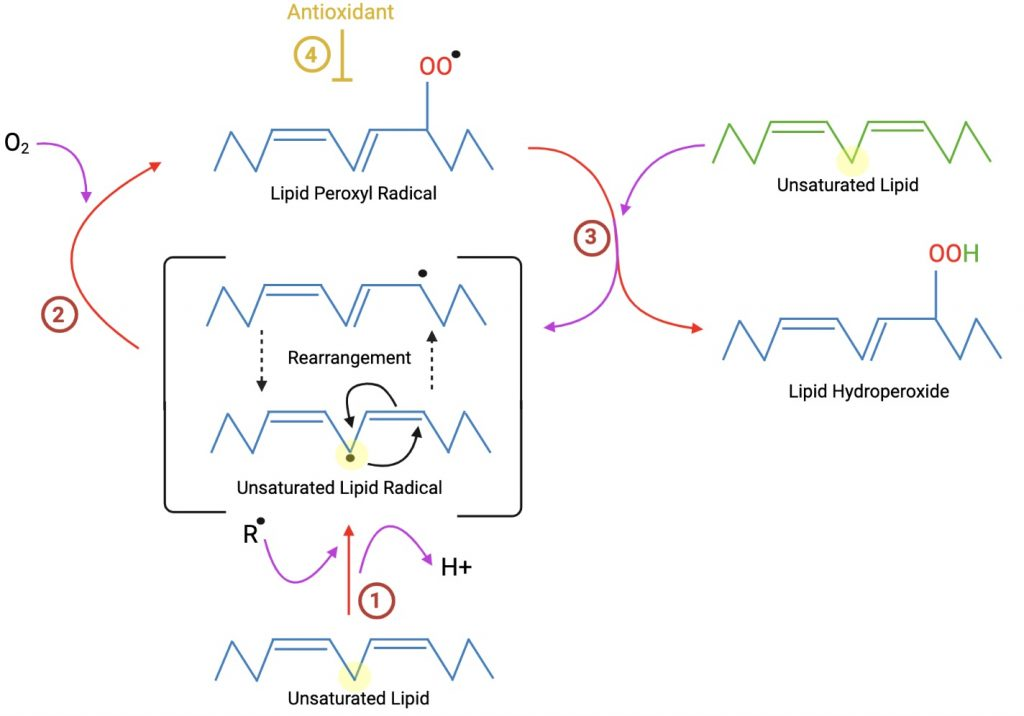
\includegraphics[width = 0.8\textwidth]{Fig/lpperox.jpg}
	\end{center}
	\caption{Lipid Peroxidation Mechanism. (1) Initiation begins when R (an \ac{ROS}) abstracts a hydrogen from the highlighted region. The carbon-centered lipid radical is stabilized by molecular rearrangement, forming a conjugated diene. (2) In propagation, lipid radicals rapidly react with oxygen to form a lipid peroxyl radical. (3) Propagation continues with the lipid peroxyl radical abstracting a hydrogen from another lipid molecule. This generates another unsaturated lipid radical as well as a lipid hydroperoxide. (4) Termination of the radical reaction occurs when antioxidants donate a hydrogen atom to the lipid peroxyl radical species, forming nonradical products.  However, termination is not possible in the absence of radical species. Therefore, propagation will continue until there is a radical sink. Figure created using BioRender and redrawn from \cite{lpperox}}\label{fig:lpperox}
\end{figure}

Accumulation of lipid peroxides disrupts the integrity of cellular membranes, particularly the lipid bilayer \citep{lppmembrane}. Membrane damage leads to the loss of compartmentalization and function within the cell, including the mitochondrion \citep{lppmito}. Eventually, the cell membrane will rupture, resulting in cell death.

Healthy mammalian cells stave off this threat in a number of ways. The primary cellular mechanism of protection against oxytosis/ferroptosis is mediated by \ac{GPX4}, a glutathione-dependent hydroperoxidase that converts lipid peroxides into non-toxic lipid alcohols \citep{gpx4}. \ac{GSH} itself, which is produced from \ac{l-CysH}, is able to neutralize \ac{ROS} present within the cell directly, playing the role of antioxidant \citep{glutath}. For an overview of the various co-dependent pathways and effects classically associated with ferroptosis, see Fig. \ref{fig:ferro_mech}.

\ac{SxC-}, an amino acid antiporter, primarily facilitates the exchange of extracellular \ac{l-Cys2} and intracellular \ac{l-Glu} across the cellular plasma membrane. Studies initially emphasized the transport of \ac{l-Cys2} influx, as in numerous cells, this process acts as a rate-limiting step for supplying intracellular \ac{l-CysH} essential for \ac{GSH} synthesis \citep{sxc-}.

% 3. **FSP1 (Ferroptosis Suppressor Protein 1)**: This gene encodes a protein that acts as a key regulator of ferroptosis by reducing coenzyme Q10, a lipid-soluble antioxidant.

Beyond these key proteins and enzymes, it has been proven that the mitochondrion plays a substantial role in ferroptosis regulation and induction, being the major compartment for cellular iron metabolism \citep{mito_ferro2}. Ferroptosis is characterized by significant morphological alterations in mitochondria such as fragmentation and cristae enlargement \citep{mito_ferro3}, is closely linked with cellular mechanisms. Interestingly, certain potent ferroptosis inhibitors demonstrate a remarkable specificity towards mitochondria \citep{mito_ferro4}. Mitochondrial shrinkage and rupture are also common terminal observations when a cell undergoes ferroptosis, since this organel is enveloped in a membrane \citep{mito_ferro}.

\begin{figure}[ht]
	\begin{center}
		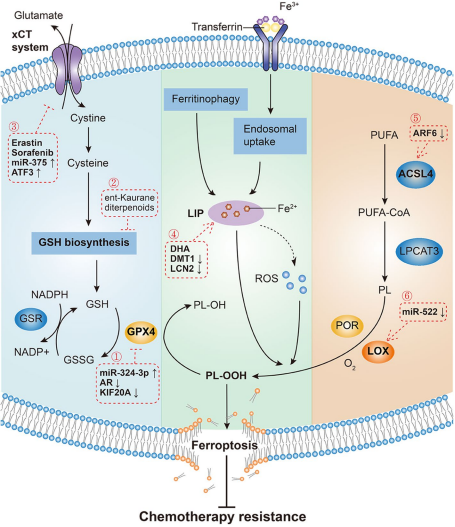
\includegraphics[width = 0.5\textwidth]{Fig/ferroptosis.png}
		\end{center}
		\caption{Overview of the various regulatory pathways associated with ferroptosis \citep{ferro_cancer}.}\label{fig:ferro_mech}
\end{figure}

\section{The Prospect of Ferroptosis in Cancer Therapy}

Cancer is the second leading cause of death worldwide, behind cardiovascular disease \citep{cancer}. Ongoing global research efforts have led to notable enhancements in cancer survival rates over the years. Despite these significant advancements in cancer treatment, including surgery, radiation therapy, chemotherapy, hormone therapy, targeted therapy, and immunotherapy \citep{therapies}, resistance to these therapies remains a prevalent challenge in clinical practice \citep{therapy_resistance}.

The phenomenon of drug resistance, where diseases develop tolerance to pharmaceutical treatments, initially emerged with antibiotic-resistant bacteria. However, this concept extends beyond bacteria to encompass various diseases, including cancer. While some resistance mechanisms are disease-specific, others, like drug efflux, occur across microbes and drug-resistant cancers, indicating evolutionary conservation. Despite initial susceptibility to chemotherapy, many cancers eventually develop resistance through mechanisms such as DNA mutations and metabolic changes, which hinder drug inhibition and promote degradation \citep{therapy_resistance2}.

The prevalence of acquired resistance to targeted therapy underscores the urgent need for effective strategies to combat drug resistance. Recent findings highlight the significant role of ferroptosis in cancer therapy, disrupting target molecules and influencing cancer progression. Furthermore, studies have indicated that leveraging ferroptosis may offer a promising avenue to overcome resistance to targeted therapy \citep{ferro_drugs}. Typically in cancer, the apoptotic pathway faces inhibition through various mechanisms, such as the overexpression of antiapoptotic proteins and the under-expression of proapoptotic proteins. These alterations often lead to intrinsic resistance to chemotherapy, a prevalent anticancer therapy. It is primarily due to ferroptosis' profile as a non-apoptotic form of \ac{RCD} that makes it an incredibly promising avenue for new therapy strategies, allowing it to circumvent many tumors' natural resilience to apoptotic induction.

In the field, ferroptosis is indeed commonly acknowledged as a tumor suppressor mechanism. Research has demonstrated that the inactivation of the p53 tumor suppression pathway, implicated in the genesis of most human cancers, is correlated with the natural suppression of ferroptosis \citep{p53}. Activation of p53 obstructs cystine uptake via the cystine/glutamate antiporter, thereby reducing intracellular \ac{GSH} levels and shielding tumor cells from ferroptosis. 

The synthesis and validation of ferroptosis inducers through various in vivo experiments underscore their potential as a viable anticancer therapy for clinical use pending extensive population validation. Consequently, numerous investigations have delved into the development of diverse inducers to trigger ferroptosis, examining its efficacy in various cancer treatment modalities including chemotherapy, immunotherapy, radiotherapy, nanotherapy, \ac{SDT}, and \ac{PDT}.

Tumor drug resistance arises from a multitude of mechanisms, with the disruption of redox homeostasis emerging as a pivotal factor. Tumor cells bolster their resilience against oxidative stress by curtailing their own production of \ac{ROS}, fostering the development of acquired drug resistance \citep{ferro_res}. Being able to predict which tumors are more inclined than others to respond well to ferroptosis induction would aid significantly in lowering the bar for targeted research and treatment.

\section{DNA Methylation and its Role in Cancer}

In mammalian cells, the process of DNA methylation predominantly involves the addition of a methyl group to the carbon-5 atom of cytosine within \ac{CpG} dinucleotides. This biochemical reaction is facilitated by three main enzymes known as \acp{DNMT}, including DNMT1, DNMT3A, DNMT3B \citep{dnmt_enzymes}. Essential for mammalian development, these enzymes facilitate the transfer of a methyl group from the universal methyl donor, \ac{SAM}, to the 5-position of cytosine residues in DNA \citep{dnmt}. Following DNA replication, the newly synthesized DNA strand lacks methylation. DNMT1 predominantly methylates the unmethylated strand of hemimethylated DNA, with DNMT3a/3b assisting in ensuring efficient propagation of DNA methylation, especially at sites overlooked by DNMT1 \citep{dnmt_enzymes}.

While \acp{DNMT} are responsible for adding methyl groups, the ten-eleven translocation (\ac{TET}) family of dioxygenases has emerged as key players in DNA demethylation. Through successive enzymatic processes, \ac{TET} enzymes can oxidize \ac{5mC} to \ac{5hmC}, and further to \ac{5fC} and \ac{5caC} \citep{tet}. This oxidation of \ac{5mC} contributes to the gradual loss of DNA methylation during cell replication. Additionally, the oxidized intermediates can be converted back to cytosine through iterative oxidation followed by base excision repair facilitated by \ac{TDG} \citep{demeth}. Together with \acp{DNMT}, these enzymes orchestrate the dynamic regulation of DNA methylation.

Methylated cytosine residues are prone to spontaneous deamination, leading to the conversion of cytosine to thymine, a transition that is often poorly repaired. Consequently, a significant portion of familial mutations and single-nucleotide polymorphisms associated with diseases are found within methylated CpG sites. Moreover, CpG residues within gene bodies or coding regions in somatic cells frequently serve as mutational hotspots, exemplified by inactivating C to T transitions in the tumor suppressor gene p53 \citep{meth_p53}.

This phenomenon also results in a diminished presence of the CpG palindrome throughout the human genome, except within regions identified as \acp{CGI}. \acp{CGI}, originally characterized by \cite{cgi}, are defined as 200-bp DNA segments with a 50\% C + G content and an observed CpG frequency exceeding the expected value of 0.6. While most CpGs undergo methylation, those within \acp{CGI} typically remain unmethylated \citep{cgi2}. \acp{CGI} are predominantly located within approximately half of all gene promoters \citep{cgi3}. Conversely, non-\ac{CGI} promoters are usually methylated and transcriptionally silent. These genes are more likely to exhibit tissue-specific expression, resulting in only a fraction of non-CGI promoters remaining unmethylated and accessible to transcription factors in each tissue type \citep{meth_chrom}.

Recent advancements in next-generation sequencing techniques applied to cancer genomes have unveiled a prevalent pattern of mutations recurring in diverse epigenetic modulators. These modulators encompass mediators of DNA methylation, covalent histone modifiers, and genes encoding subunits of chromatin remodelers \citep{meth_cancer}. The aberrant functioning of these pivotal epigenetic regulators leads to the dysregulation of gene expression and is implicated in a myriad of malignancies, spanning various cancer types \citep{meth_cancer2}.

\section{DNA Methylation Detection Techniques}

Bisulfite genomic sequencing stands as the benchmark technology for detecting DNA methylation due to its ability to offer qualitative, quantitative, and highly efficient insights into identifying 5-methylcytosine at single base-pair resolution. Initially pioneered by \cite{bisulfite_ori}, this method capitalizes on the discovery that the amination reactions of cytosine and \ac{5mC} yield markedly distinct outcomes following treatment with sodium bisulfite.

In this context, cytosines present in single-stranded DNA undergo conversion into uracil residues, which are subsequently recognized as thymine during PCR amplification and sequencing. However, \acp{5mC} remain unaffected by this conversion, retaining their cytosine identity and enabling the distinction between methylated and unmethylated cytosines \citep{bisulfite2}. 

Following bisulfite treatment, a subsequent PCR step becomes imperative to ascertain the methylation status at specific loci, employing methylation-specific primers. The actual methylation status can then be determined through either direct sequencing of PCR products (for the detection of average methylation status) or sub-cloning sequencing (for the detection of the distribution of methylation patterns at the single-molecule level) \citep{bisulfite2}.

Despite being the current gold standard, bisulfite sequencing is not without its flaws. Understanding bisulfite-treated DNA data requires careful consideration of two types of conversion errors: failed conversion and inappropriate conversion. Failed conversion, extensively studied, arises when an unmethylated cytosine fails to deaminate, resulting in its appearance as methylated in sequencing data. In mammalian somatic cells, where 5-methylcytosine primarily occurs at CpG cytosines, the frequency of failed conversion is indicated by the proportion of non-CpG cytosines appearing as cytosines in sequence data \citep{bisulfite_failed_conv}. Ignoring failed conversion in data analysis can inflate methylation density estimates and impede the determination of DNA methyltransferase sequence motif preferences.

Inappropriate conversion, the second type of error, occurs when a methylated cytosine undergoes deamination, yielding thymine \citep{bisulfite_inappr_conv}. Similar to uracils resulting from cytosine deamination, thymine pairs with adenine during PCR. Consequently, 5-methylcytosines subjected to inappropriate conversion are misinterpreted as unmethylated. Failure to account for inappropriate conversion leads to underestimation of genomic methylation densities. However, if the frequency of inappropriate conversion is known, it can be integrated as a parameter in data analysis. Therefore, information on both failed and inappropriate conversion frequencies is crucial for drawing meaningful insights from detailed DNA methylation patterns.

In addressing the limitations of bisulfite sequencing, new techniques have emerged despite its status as the gold standard for detecting methylation marks. These limitations encompass the aforementioned confounding effects of bisulfite treatment on DNA methylation, alongside the challenge of distinguishing between DNA methylation and hydroxylation \citep{ont_vs_bisulfite}. In light of these considerations, we advocate for the utilization of Nanopore sequencing as a promising alternative for identifying methylation marks.

Nanopore sequencing is a next-generation sequencing technology that enables the real-time analysis of DNA or RNA molecules as they pass through a nanoscale pore. This technique is based on the principle that as a DNA strand translocates through a nanopore, changes in the electrical current can be measured and used to deduce the sequence of the DNA molecule \cite{ont}. 

The raw electrical signal is translated into DNA sequence information through a process called basecalling. DNA methylation involves the addition of a methyl group to a cytosine base, commonly referred to as a 5-methylcytosine. Nanopore sequencing can detect these modifications as changes in the electrical current during translocation using specialized algorithms and basecallers (Fig. \ref{ont_epi}).

\begin{figure}[ht]
	\begin{center}
		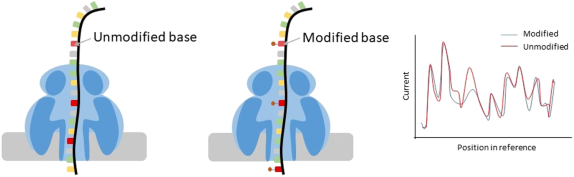
\includegraphics[width = \textwidth]{Fig/ont_epi.png}
	\end{center}
	\caption{Direct base modification detection with \ac{ONT}.}\label{ont_epi}
\end{figure}

One of the key advantages of nanopore sequencing is its ability to generate long reads, providing information about entire genomic regions in a single continuous sequence. Short-read sequencing offers a cost-effective and accurate solution, bolstered by a diverse array of analysis tools and pipelines \citep{short_reads}. However, the vast range of lengths spanning natural nucleic acid polymers, extending over eight orders of magnitude, presents a challenge when sequencing them in short amplified fragments, hindering the reconstruction and quantification of the original molecules. 

Long reads, on the other hand, hold the potential to enhance de novo assembly, ensure mapping accuracy, facilitate transcript isoform identification, and enable the detection of structural variants. Moreover, the sequencing of native molecules, both DNA and RNA, using long reads, eliminates amplification bias while retaining base modifications \citep{long_read_adv}. These capabilities, coupled with ongoing advancements in accuracy, throughput, and cost reduction, are establishing long-read sequencing as a viable option for a wide spectrum of genomic applications in both model and non-model organisms \citep{long_read_adv2}.

Adaptive sampling is a feature that helps optimize the sequencing process by adjusting data collection parameters in real-time based on the characteristics of the DNA being sequenced. The system monitors various parameters such as the quality of the signal, the speed at which the DNA is translocating through the nanopore, and other relevant metrics \citep{ont_as}. The software requires a user to upload a file of whitelisted reference sequences, and the system can be set to either deplete or enrich for these on a specified set of channels. 

In order to achieve this, the software basecalls the first few hundred bases of each read and compares it with the target reference sequences. Matching or unmatching sequences are rejected, depending on whether the software is set to enrich or deplete. By using this, coverage of our genes of interest is enriched, greatly reducing noise.